%\documentclass[12pt,letterpaper]{article}
\documentclass[12pt]{amsart}

\usepackage[left=1in, right=1in, top=.5in, bottom=.5in]{geometry}
\usepackage{latexsym,amssymb,amsmath,amsthm,amsopn,verbatim, mathpazo, graphicx, lmodern, hyperref, color, subcaption, ulem, pdfpages}
%\usepackage{latexsym,amssymb,amsmath,amsthm,amsopn,verbatim, mathpazo, graphicx}
\newcommand{\vs}{\vskip.5cm}
\newcommand{\hs}{\hskip1cm}
\newcommand{\ds}{\displaystyle}
\setlength{\parindent}{0pt}


\usepackage[T1]{fontenc}
\usepackage{libertine}
\renewcommand*\familydefault{\sfdefault}  %% Only if the base font of the document is to be sans serif


\newtheorem{theorem}{Theorem}[section]
\newtheorem{corollary}{Corollary}[theorem]
\newtheorem{lemma}[theorem]{Lemma}
\newtheorem{definition}[theorem]{Definition}
\newtheorem{example}[theorem]{Example}

\newcommand\indep{\protect\mathpalette{\protect\independenT}{\perp}}
\def\independenT#1#2{\mathrel{\rlap{$#1#2$}\mkern2mu{#1#2}}}
\newcommand{\m}{\mu}
\newcommand{\s}{\sigma}
\newcommand{\gl}{\lambda}
\newcommand{\bP}{\mathbb{P}}
\newcommand{\bE}{\mathbb{E}}
\newcommand{\xb}{\bar{x}}
\newcommand{\ph}{\hat{p}}


\begin{document}


%----------------------------------------------------------------------------
\setcounter{section}{3}
\setcounter{subsection}{2}
%\setcounter{theorem}{1}
Day 7 BSTA 511/611
{\huge  
\section*{Chapter 3: Distributions of Random Variables (Part 2)}
}

%----------------------------------------------------------------------------


%----------------------------------------------------------------------------
{\large 
%----------------------------------------------------------------------------

\emph{Day 7 topics}:

Section 3.3: Normal distribution  \newline
Section 3.4: Poisson distribution

\hrulefill

%----------------------------------------------------------------------------
%\begin{example}  \textbf{text.} \newline
%
%\begin{enumerate}
%\item 
%
%\vspace{2cm}
%
%\item 
%
%\vspace{2cm}
%
%\item 
%
%\vspace{2cm}
%\end{enumerate}
%\end{example} 

%\newpage
%----------------------------------------------------------------------------
%\tableofcontents



% \newpage
%----------------------------------------------------------------------------
%\vspace{1cm}


\vspace{.5cm}

%Section 3.3
\subsection{Normal distribution} $\ $ \newline

A random variable $X$ is modeled with a normal distribution if:
\begin{itemize}
\item shape: symmetric, unimodal bell curve
\item center: mean $\m$
\item spread (variability): standard deviation $\s$
\item Curve is determined by the formula $f(x) = \frac{e^{-\frac{(x-\m)^2}{2\s^2}}}{\s\sqrt{2\pi}}$, for $-\infty < x< \infty$.

%\item 
\end{itemize}

\begin{figure}[h!]
  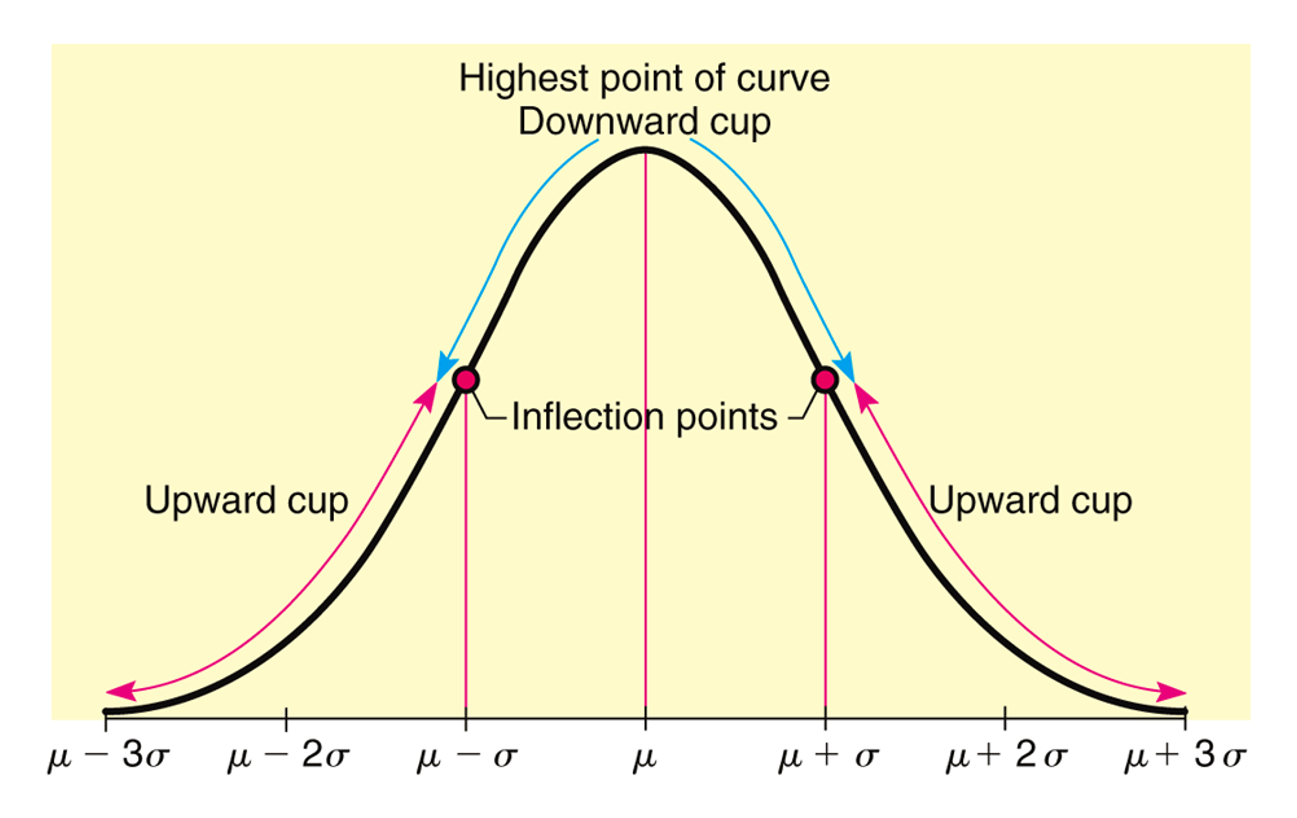
\includegraphics[width=3.8in]{img/normal_curve_Brase.png}
  \caption{Normal (Gaussian) distribution}
  \label{fig:normal}
\end{figure}

%%delete
%\color{blue}
%$X\sim N(\m,\s)$, Total area =1;  L: $\m=0, \s=2, 5$, R: $\m=-1, \s=4$, $\m=3, \s=2$
%\color{black}

\begin{figure}[h!]
  \centering
  \begin{subfigure}[b]{0.47\linewidth}
    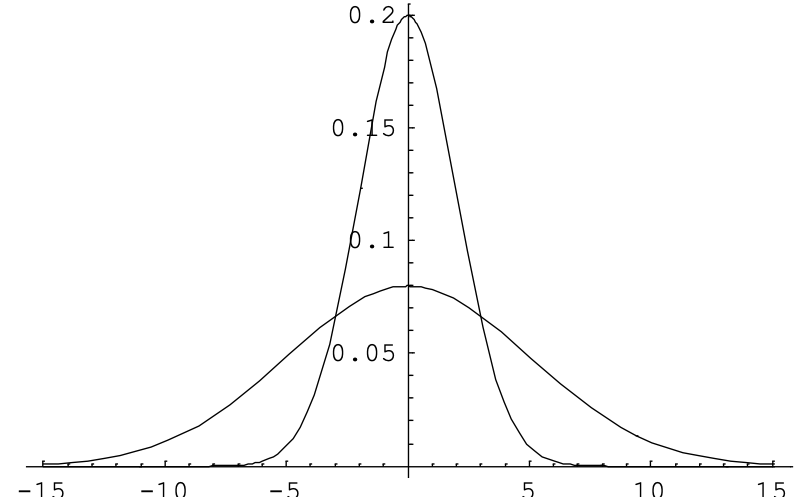
\includegraphics[width=\linewidth]{img/normal_curves_compare_v1.png}
%    \caption{Coffee.}
  \end{subfigure}
  \begin{subfigure}[b]{0.52\linewidth}
    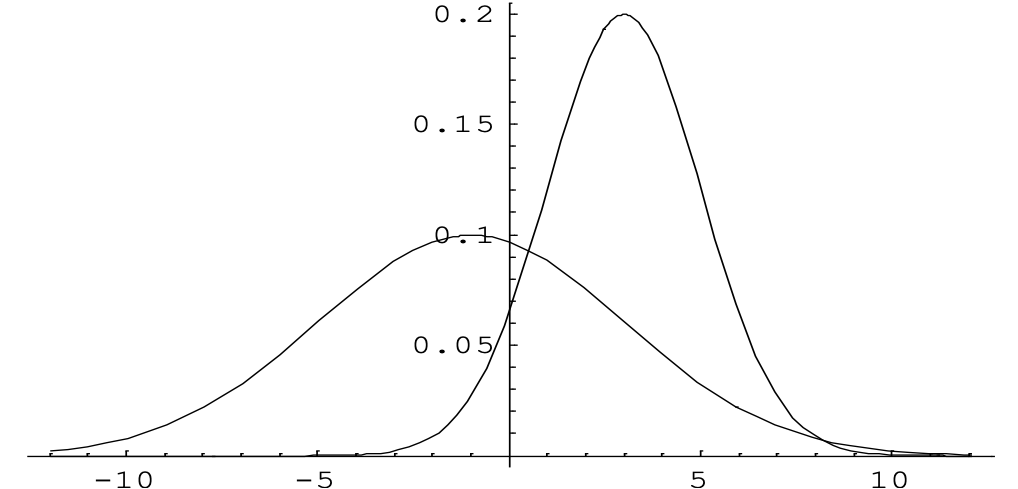
\includegraphics[width=\linewidth]{img/normal_curves_compare_v2.png}
%    \caption{More coffee.}
  \end{subfigure}
  \caption{What are the means and standard deviations?}
%  \label{fig:coffee}
\end{figure}


\newpage
%----------------------------------------------------------------------------

\textbf{The Empirical Rule} (a.k.a. the 68-95-99.7 rule) \newline

For a normal distribution: 
\begin{itemize}
\item 68\% of observations are within one standard deviation (SD) of the mean
\item 95\% are within two SD’s
\item 99.7\% are within three SD’s
\end{itemize}


%figure from oi_biostat
\begin{figure}[h!]
  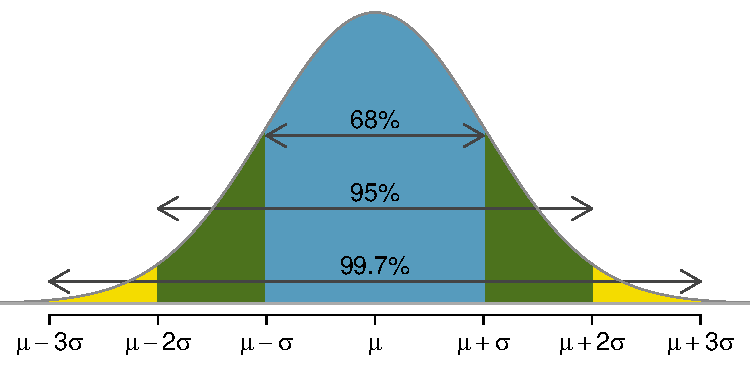
\includegraphics[width=5in]{img/6895997.pdf}
  \caption{Empirical Rule (a.k.a. the 68-95-99.7 rule)}
  \label{fig:normal}
\end{figure}


The empirical rule is useful for \textit{estimating} probabilities.

\vspace{1cm}
%----------------------------------------------------------------------------

\textbf{Standard Normal Distribution} \newline

\begin{itemize}
\item A \textbf{standard} normal r.v. has mean 0 and standard deviation 1.
\item We denote standard normal r.v.'s with the letter $Z$.
\end{itemize}

%%delete
%\color{blue}
%$$Z\sim N(\m=0,\s=1)$$
%
%\begin{itemize}
%\item Sketch Z curve
%\item sd determined by POI
%\item estimate probabilities via empirical rule
%\item 50/50
%\item 2.35\%, 13.5\%, 34\%
%\item $\bP(Z<0) = .0235 $
%\item $\bP(Z<-2) = .0235 $
%\item $\bP(Z> 1) = .0235 + .135 = 0.1585$ 
%\end{itemize}
%
%
%\color{black}



\newpage
%----------------------------------------------------------------------------

%----------------------------------------------------------------------------

\textbf{Calculating Probabilities for a Standard Normal Distribution} \newline

Three ways to calculate probabilities from a normal distribution:

\begin{enumerate}
\item \sout{Calculus}
\item Normal probability table
	\begin{itemize}
	\item The textbook has a normal probability table in Appendix B.1, which is included as the next two pages.
	\end{itemize}
\item R
	\begin{itemize}
	\item $\bP(Z\leq q)$ = \begin{verbatim}pnorm(q, mean = 0, sd = 1, lower.tail = TRUE)\end{verbatim}
	\end{itemize}	
\end{enumerate}

\vspace{.5cm}






%----------------------------------------------------------------------------
\begin{example}  \textbf{Calculating standard normal probabilities practice} \newline
Let $Z$ be a standard normal random variable, $Z\sim N(\m=0,\s=1)$.\newline
Calculate the following probabilities. Include sketches of the normal curves with the probability areas shaded in.

\begin{enumerate}
\item $\bP( Z < 2.67 ) $
%%delete
%\color{blue}
%$$\bP( Z < 2.67 )= 0.9962$$
%\begin{verbatim}
%pnorm(2.67) = 0.9962074                                          
%\end{verbatim}
%\color{black}

%\vspace{2cm}
\vfill

\item $\bP( Z > -0.37 ) $
%%delete
%\color{blue}
%$$\bP( Z > -0.37 ) = 1 - \bP( Z < -0.37 ) =  1 - 0.3557 = 0.6443$$
%
%\begin{verbatim}
%pnorm(-0.37, lower.tail = F) = 0.6443088
%\end{verbatim}
%\color{black}

%\vspace{2cm}
\vfill


\item $\bP( -2.18 < Z < 2.46 )$
%%delete
%\color{blue}
%$$= \bP( Z < 2.46 ) - \bP( Z < -2.18)
%= 0.9931 - 0.0146
%= 0.9785$$
%
%\begin{verbatim}
%pnorm(2.46) - pnorm(-2.18) =  0.9784244
%\end{verbatim}
%\color{black}

%\vspace{2cm}
\vfill


\item $\bP(Z = 1.53 ) $
%%delete
%\color{blue}
%$$\bP(Z = 1.53 ) 
%= \bP( Z < 1.53 ) - \bP( Z < 1.53)
%= 0.9370 - 0.9370 = 0$$
%\color{black}

\end{enumerate}
%\vspace{1cm}


%\vspace{1cm}
\end{example} 


\newpage
%----------------------------------------------------------------------------
%\usepackage[final]{pdfpages}
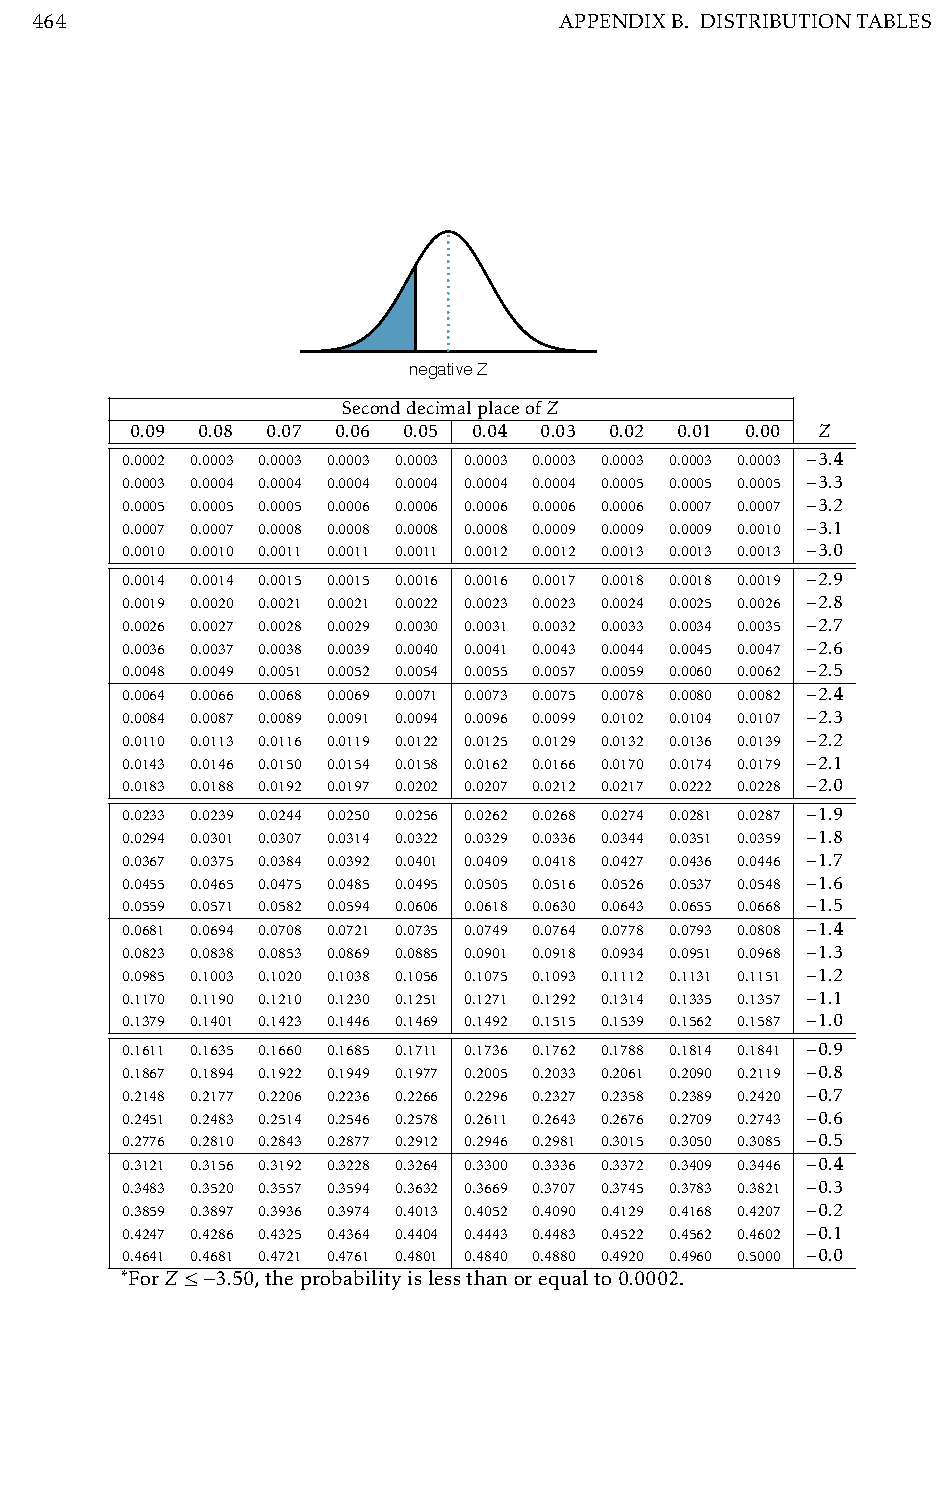
\includepdf[pages=-]{img/Appendix_z_tables.pdf}   % for the entire file



\newpage
%----------------------------------------------------------------------------
\textbf{Calculating Probabilities for a General Normal Distribution} \newline

%----------------------------------------------------------------------------
\begin{example}  Let $X$ be a normal r.v. with mean 8 and standard deviation 2.  \newline
Calculate $\bP(X>10)$.
\end{example} 

%%delete
%\color{blue}
%Blue areas (probabilities) do not change via transformation!
%\color{black}

%figure from Brase
\begin{figure}[h!]
  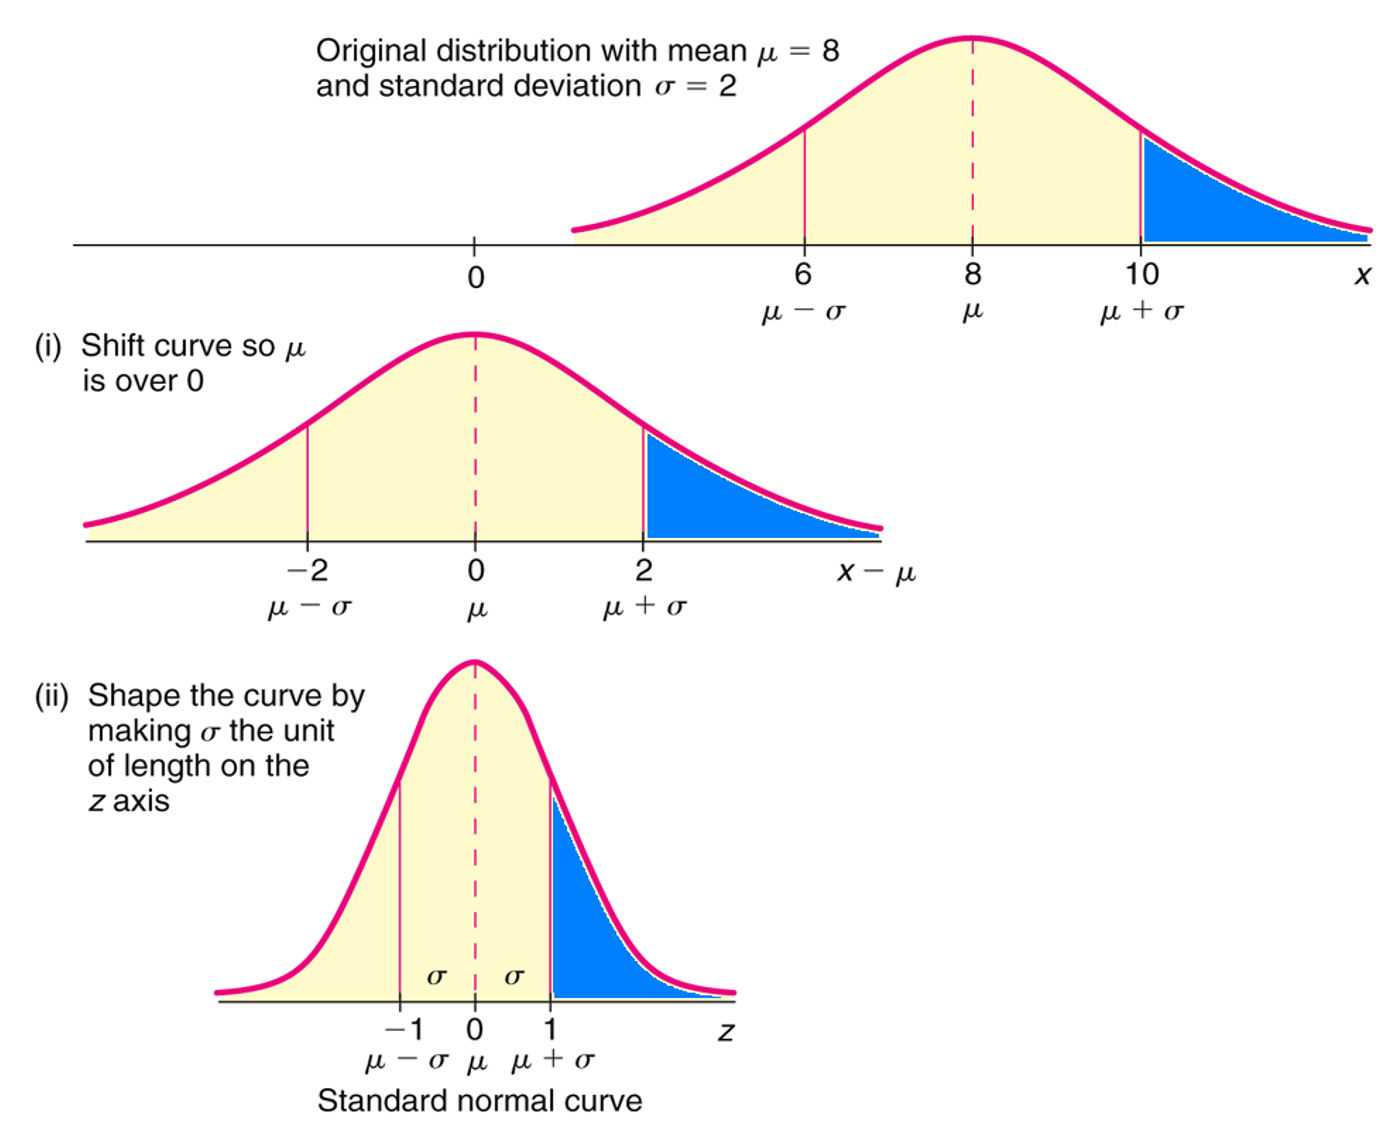
\includegraphics[width=5in]{img/X_to_Z_transformation_Brase.png}
  \caption{Transformation from general normal $X$ to standard normal $Z$}
%  \label{fig:normal}
\end{figure}


%----------------------------------------------------------------------------
\textbf{Z-scores} \newline

%%delete
%\color{blue}
%$$z = \frac{x-\m}{\s}$$
%
%\begin{itemize}
%\item $\bP( X > 10 ) = \bP( Z >  \frac{10-8}{2}) = \bP( Z >  1) = 1 - \bP( Z <  1) = 1- 0.8413 = 0.1587$
%\item pnorm(1, lower.tail = F) = 0.1586553
%\item pnorm(10, mean = 8, sd =2, lower.tail = F)
%\end{itemize}
%
%\color{black}

\vfill 

\begin{itemize}
\item The $Z$-score of an observation quantifies how far the observation is from the mean, in units of standard deviation(s). 
\item For example, if an observation has $Z$-score $z = 3.4$, then the observation is 3.4 standard deviations above the mean.
\end{itemize}



\newpage
%----------------------------------------------------------------------------
\begin{example}  \textbf{DBP} \newline
Suppose the distribution of diastolic blood pressure (DBP) in 35- to 44-year old men is normally distributed with mean 80 mm Hg and variance 144 mm Hg. 

\begin{enumerate}
\item Mild hypertension is when the DBP is between 90 and 99 mm Hg. What proportion of this population has mild hypertension?

%%delete
%\color{blue}
%$$\bP( 90 < X < 99 ) = \bP\Big( \frac{90-80}{\sqrt{144}} < Z <  \frac{99-80}{12}\Big) = \bP( 0.83 < Z <  1.58) $$
%$$ = \bP(Z <  1.58)  - \bP( Z < 0.83)  = 0.9429 - 0.7967 = 0.1462
%$$
%pnorm(99, m = 80, s = 12) - pnorm(90, m = 80, s = 12) = 0.1456556
%
%\color{black}

\vfill

\item What is the $10^{th}$ percentile of the DBP distribution?

%%delete
%\color{blue}
%$$x = \m +z\s = 80 + 12z$$
%Look up 0.10 in body of table. Get $z = -1.28$:DBP
%$$ \bP(Z <  -1.29) = 0.0985 ~~(diff = 0.0015)$$
%$$ \bP(Z <  -1.28) = 0.1003 ~~(diff = 0.0003)$$
%$$x = \m +z\s = 80 + 12(-1.28) = 64.64~ \textrm{mmHg}$$
%
%\begin{verbatim}qnorm(p, mean = 0, sd = 1, lower.tail = TRUE)
%\end{verbatim}
%qnorm(.10, m = 80, s = 12) =  64.62138
%\color{black}

\vfill

\item What is the $95^{th}$ percentile of the DBP distribution?

%%delete
%\color{blue}
%$$x = \m +z\s = 80 + 12z$$
%Look up 0.95 in body of table. Get $z = 1.645$ (average):
%
%$$ \bP(Z <  1.64) = 0.9495 ~~(diff = 0.0005)$$
%$$ \bP(Z <  1.65) = 0.9505~~(diff = 0.0005)$$
%$$x = \m +z\s = 80 + 12(1.645) = 99.74~ \textrm{mmHg}$$
%
%qnorm(.95, m = 80, s = 12) =  99.73824 \newline
%= qnorm(.05, m = 80, s = 12, lower.tail = F)
%\color{black}


\vfill
\end{enumerate}

\end{example} 


\newpage
%----------------------------------------------------------------------------
\textbf{Normal approximation of the binomial distribution} \newline


\begin{itemize}
\item Recall that a binomial random variable $X$ counts the total number of successes in $n$ independent trials, each with probability $p$ of a success. 
\item Probability function for $x = 0, 1, ..., n$ :
$$P(X = k) = {n\choose k}p^k(1-p)^{n-k} = \frac{n!}{k!(n-k)!}p^k(1-p)^{n-k}$$
\item Tedious to compute for large number of trails ($n$), although doable with software like R. 
\item As $n$ gets big though, the distribution shape of a binomial r.v. gets more and more symmetric, and can be \textit{approximated by a normal distribution}.
\end{itemize}




%figure from io_biostats
\begin{figure}[h!]
  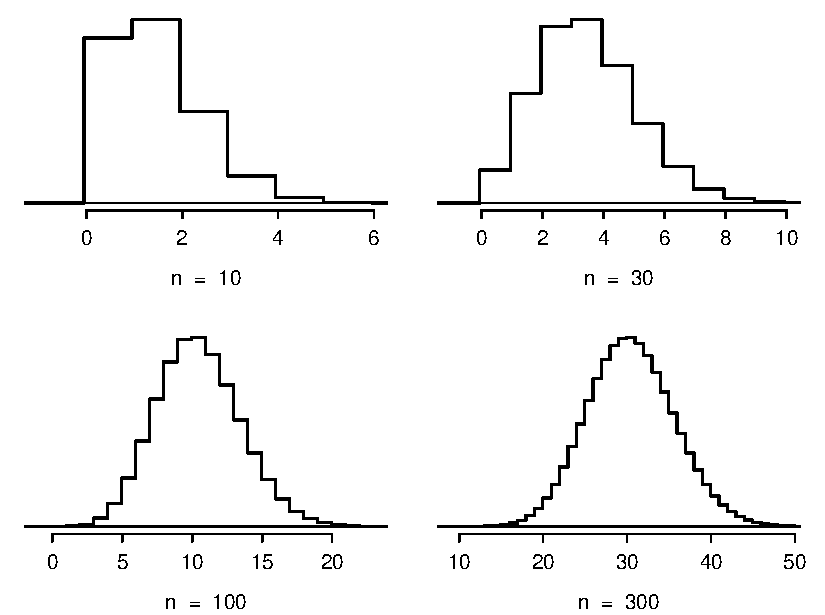
\includegraphics[width=5in]{img/fourBinomialModelsShowingApproxToNormal.pdf}
  \caption{Binomial distribution histograms for varying $n$ when $p=0.10$}
%  \label{fig:normal}
\end{figure}



\begin{theorem}\textbf{Normal approximation of the binomial distribution}\newline
The binomial distribution with probability of success $p$ is nearly normal when the sample size $n$ is sufficiently large such that $np \geq 10$ and $n(1-p)\geq 10$. \newline
The approximate normal distribution has parameters corresponding to the mean and standard deviation of the binomial distribution:
\begin{align*}
\mu &= np
&&\sigma= \sqrt{np(1-p)}
\end{align*}
\end{theorem}


\newpage
%----------------------------------------------------------------------------
\begin{example}\label{VaccBinom10}  \textbf{Vaccinated people testing positive for Covid-19 (revisited)} \newline
About 25\% of people that test positive for Covid-19 are vaccinated for Covid-19.\newline
Suppose 100 people have tested positive for Covid-19 (independently of each other). \newline
Let $X$ denote the number of people that are vaccinated amongst the 100 that tested positive.\newline
What is the probability that fewer than 20 of the people that tested positive are vaccinated?
%figure from R
\begin{figure}[h!]
  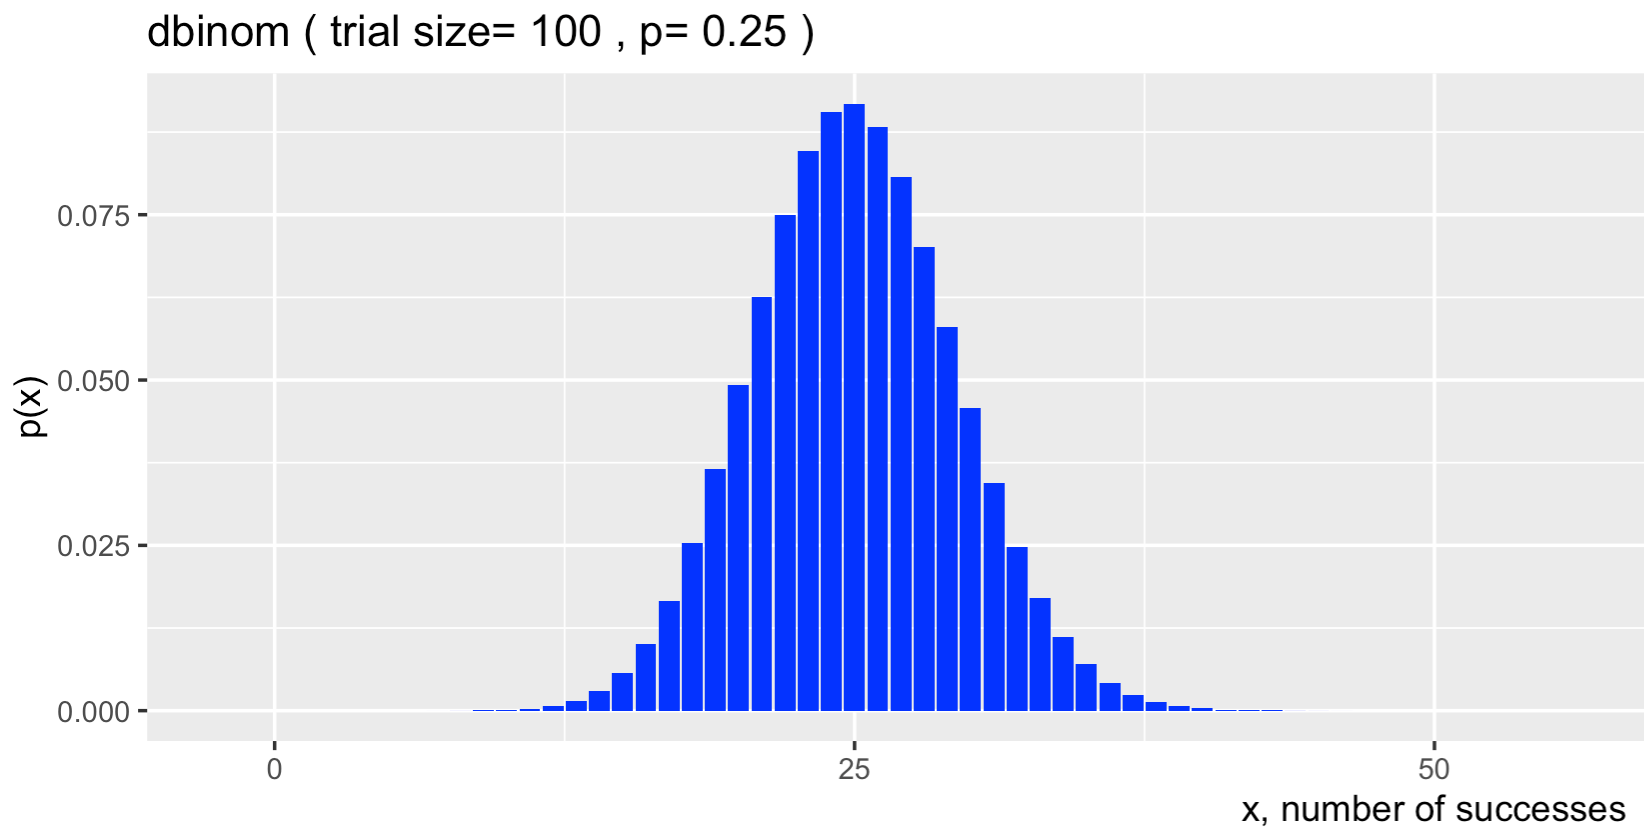
\includegraphics[width=4in]{img/binom_n100_p25_crop.png}
%  \caption{Binomial distribution histogram for $n=1000$ and $p=0.25$}
%  \label{fig:normal}
\end{figure}



\begin{enumerate}
\item Calculate exact probability.
%%delete
%\color{blue}
%$$
%P(X <  20) = P(X \leq 19) = \sum_{k=0}^{19} {100\choose k}0.25^k(0.75)^{100-k} 
%$$
%pbinom(19, size=100, prob = .25, lower.tail = TRUE)= 0.09953041
%
%\color{black}

%\vfill

\vspace{4cm}

\item Calculate approximate probability.

%%delete
%\color{blue}
%$$\m = np = 100(0.25) = 25$$ 
%$$\s = \sqrt{npq} = \sqrt{100(0.25)(0.75)} = 4.330127$$
%Check conditions: $np = 25 \geq 10, n(1-p) = 75 \geq 10$\newline
%CONTINUITY CORRECTION!!!!
%$$
%P(X <  20) = P(X \leq 19.5) = \bP\Big( Z <  \frac{19.5-250}{4.33}\Big) = \bP(  Z <  -1.27) = 0.1020
%$$
%pnorm(19.5, m = 25, s = 4.330127) =  0.1020119\newline
%Without CC:\newline
%pnorm(19, m = 25, s = 4.330127) =  0.08292833\newline
%pnorm(20, m = 25, s = 4.330127) =  0.1241065
%
%\color{black}

\end{enumerate}

\end{example} 


\newpage
%----------------------------------------------------------------------------
%Section 3.4
\subsection{Poisson distribution}

\vspace{.5cm}

\begin{itemize}
\item Discrete distribution
\item Used to model count data (\# of successes), especially for rare events
\item Used to approximate binomial distribution when $n$ is large and $p$ is small
\end{itemize}

%----------------------------------------------------------------------------
\vspace{.5cm}

\begin{definition}{Distribution of a \textbf{Poisson} random variable.} \newline
Let $X$ be the total number of successes in an interval (such as time) with an average success rate $\lambda$. \newline
Then probability of observing exactly $k$ successes in a unit interval is
%%delete
%\color{blue}
%$$
%P(X = k) = \frac{e^{-\lambda}(\lambda)^{k}}{k!},~\textrm{for}~ k = 0, 1, 2, \dots
%$$
%\color{black}
\vspace{3cm}
\end{definition}


%\vspace{.5cm}
\begin{itemize}
\item The parameter of a Poisson distribution is $\lambda$. 
\item If a r.v. $X$ is modeled by a Poisson distribution, then we write in shorthand  
\vspace{1cm}
%%delete
%\color{blue}
%$$X \sim \textrm{Pois}(\lambda)$$
%\color{black}
\end{itemize}

%----------------------------------------------------------------------------
\begin{theorem}{Mean and SD of a Poisson r.v.} \newline
If $X$ is a Poisson r.v. with parameter $\lambda$, then 

%%delete
%\color{blue}
%$$\mu = \mathbb{E}(X) = \lambda$$
%$$\sigma^2= Var(X) = \lambda$$
%$$\sigma = SD(X) =  \sqrt{\lambda}$$
%\color{black}
\vspace{1cm}


\end{theorem}

\newpage
%----------------------------------------------------------------------------
\begin{example}  \textbf{Typhoid fever} \newline
Suppose there are on average 5 deaths per year from typhoid fever over a 1-year period. 

%figure from R
\begin{figure}[h!]
  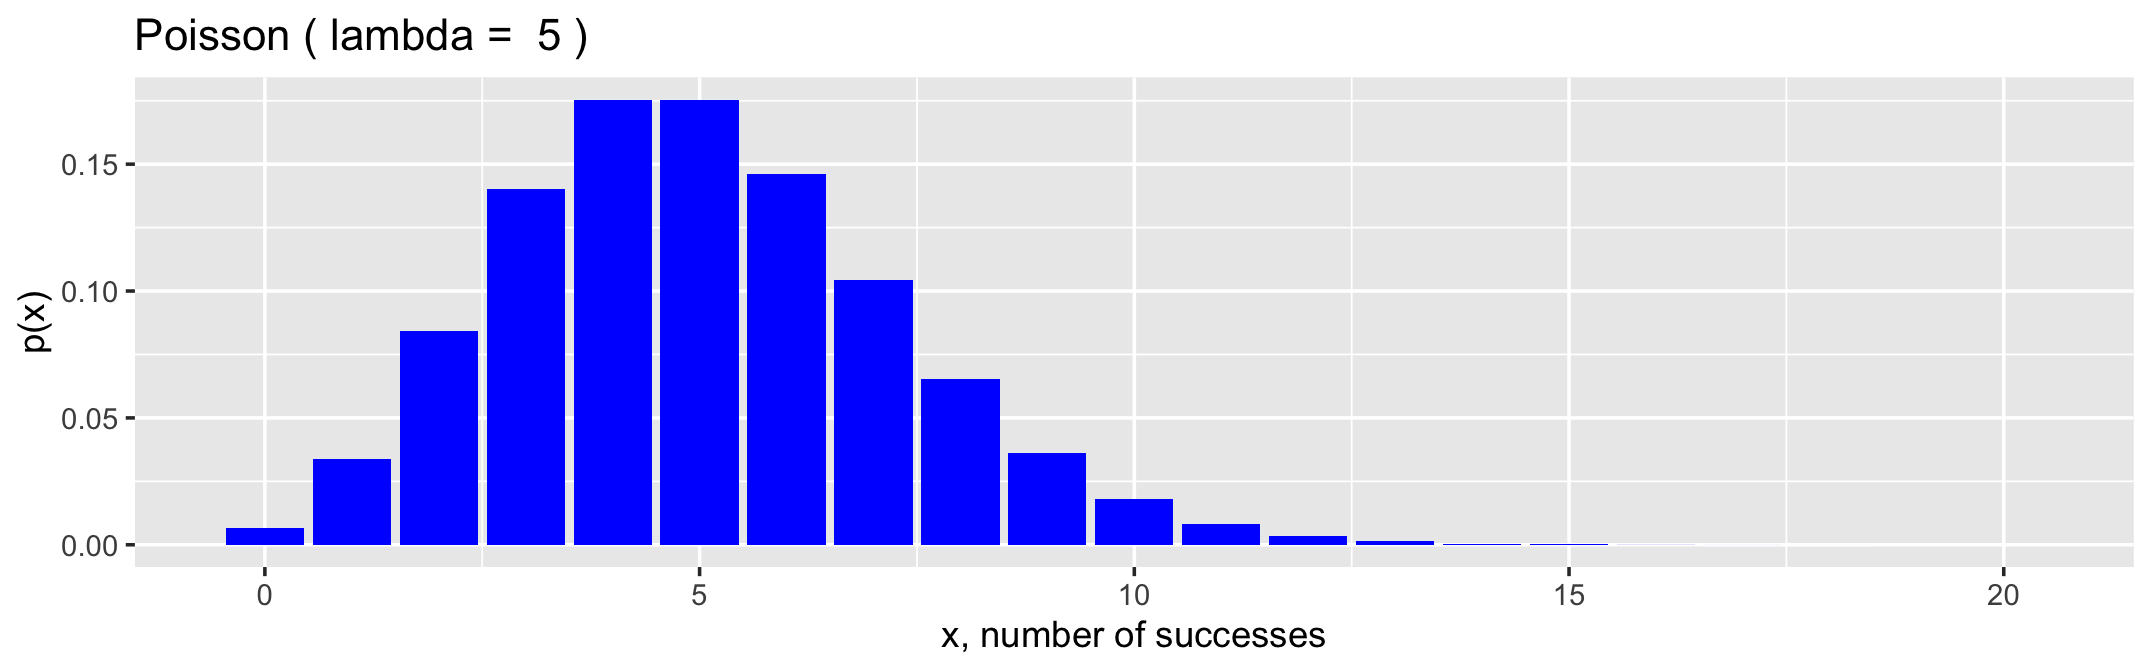
\includegraphics[width=5in]{img/Poisson_L5.png}
%  \caption{Binomial distribution histogram for $n=1000$ and $p=0.25$}
%  \label{fig:normal}
\end{figure}


\begin{enumerate}
\item What is the probability of 3 deaths in a year?

%%delete
%\color{blue}
%$$\bP(X = 3) = \frac{e^{-5}(5)^{3}}{3!}  = 0.1403739$$
%$exp(-L)*(L^k)/factorial(k)$ \newline
%dpois(x=3, lambda=5)
%\color{black}

\vfill
\item What is the probability of 2 deaths in 0.5 years?

%%delete
%\color{blue}
%$$ \lambda_{t=0.5} = \lambda\cdot t = 5*0.5 = 2.5$$
%$$\bP(X = 2) = \frac{e^{-2.5}(2.5)^{2}}{2!}  = 0.2565156$$
%dpois(x=2, lambda=2.5)
%\color{black}

\vfill

\item What is the probability of more than 12 deaths in 2 years?

%%delete
%\color{blue}
%$$ \lambda_{t=2} = \lambda \cdot t = 5\cdot2 = 10$$
%$$\bP(X > 12) = \bP(X \geq 13) = \sum_{k=13}^{\infty}\frac{e^{-10}(10)^{k}}{k!}  = 0.2084435$$
%$\bP(X > 12)$ = ppois(q=12, lambda=10, lower.tail=F) = 0.2084435 \newline
%$1 - \bP(X \leq 12)$ = 1 - ppois(q=12, lambda=10, lower.tail=T) = 0.2084435
%\color{black}

\vfill
\end{enumerate}


\end{example} 
	
\newpage
%----------------------------------------------------------------------------


%----------------------------------------------------------------------------
\begin{example}  \textbf{Cleft palate} \newline
About 1 in every 1,700 babies is born with cleft palate in the United States. Find the probability that there are 2 babies born with cleft palates amongst the next 3000 births at OHSU. 


\begin{enumerate}
\item Calculate exact probability.
%%delete
%\color{blue}
%$$X\sim Binom(n = 3000, p = 1/1700 = 0.0006)$$
%$$
%P(X =  2) = {3000\choose 2}0.0006^2(0.9994)^{2998} 
%$$
%dbinom(2, size=3000, prob = 1/1700) = 0.2667187
%
%\color{black}

\vfill

%\vspace{2cm}

\item Calculate approximate probability.

%%delete
%\color{blue}
%Rule of thumb: $\frac{1}{10} \leq npq \leq 10$
%$$X\sim Poiss(\lambda = np = 3000\cdot1/1700 = 1.764706)$$
%
%Check conditions: $\frac{1}{10} \leq npq = 1.763668 \leq 10$\newline
%
%$$\bP(X = 2) = \frac{e^{-1.76}(1.76)^{2}}{2!}  =0.2664631$$
%dpois(x=2, lambda=1.76) =  0.2664631
%
%\color{black}
\vfill

\end{enumerate}


\end{example} 


%----------------------------------------------------------------------------
}  % end large font
%----------------------------------------------------------------------------



\end{document}




